\chapter{Design}

\section{Overall System Design}

\subsection{Short description of the main parts of the system}
	The system contains three main elements: The subsystem for managing meetings, the subsystem for managing referral tickets and the subsystem for managing resources and accounting. The meeting management subsystem will contain a record of all the meetings for each member of the staff team, therefore as part of the global system, there will be a representation of the staff team and anyone who might be involved in any meetings. This subsystem will also be responsible for the reminding the users of their meetings and informing users when they've been invited to a meeting.
	The next subsystem is the system for managing support and referral tickets, this will automatically pass the ticket on to whoever is on the rota to deal with that ticket at the given time. The tickets will be listed in order of priority, which is set when they're submitted, the priority will increase with time to ensure that nothing is ignored for too long as often the issues that would be reported are very time sensitive. The tickets will be kept securely in an encrypted section of the database, and each individual ticket will only be accessible by people for whom it is relevant to ensure confidentiality and compliance with various laws concerning such information.
	The third subsystem, designed for managing the material resources within the Church will consist of a record of all of the finite resources that the Church regularly purchases and sells, the subsystem will also keep track of the money throughput.
	Because many of the people who would operate this system will not be trained nor contractually obliged to give a satisfactory quality of service, the security and access rights components of the system are of paramount importance, not only to prevent breaches in confidentiality but also to ensure that nobody is confused when the interface is more complicated than necessary therefore the system needs to determine which parts of the system are relevant to a particular person and only show them those parts.
\subsection{System flowcharts showing an overview of the complete system}

\section{User Interface Designs}
	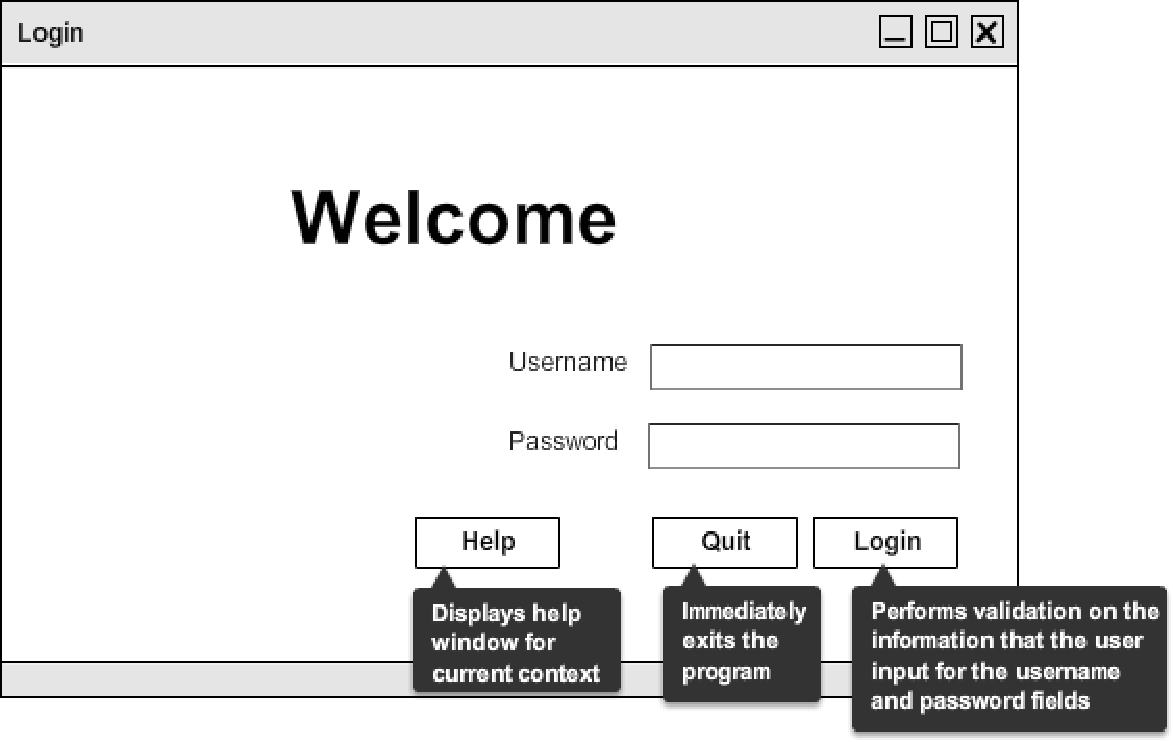
\includepdf{wireframe.pdf}
	% Put the mockflow PDF here

\section{Hardware Specification}
	The client software will have the same requirements as the python standard for 3.4 which are:
	- 2.5Gib of Disk space


\section{Program Structure}

\subsection{Top-down design structure charts}

% TODO: Include the diagrams from draw.io here

\subsection{Algorithms in pseudo-code for each data transformation process}

% TODO: Use the diargams to write some pseudo-code

\subsection{Object Diagrams}

% TODO: Remember to complete this in the analysis section

\subsection{Class Definitions}

% TODO: Define the software objects based on the ER diagrams.

%TODO: Actuall redo my entity relationship diagram
	\begin{figure}[H]
		\inlcudegraphics[width=\textwidth]{./Design/diagrams/era.jpg}
	\end{figure}

\section{Prototyping}
	\begin{figure}[H]
		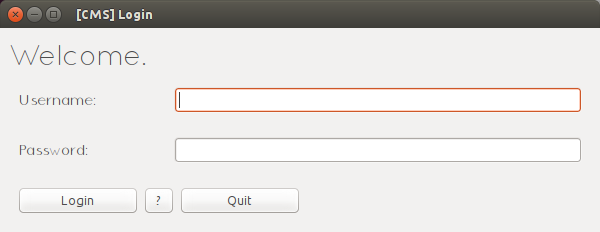
\includegraphics[width=\textwidth]{./Design/proto/1.png}
	\end{figure}
	\begin{figure}[H]
		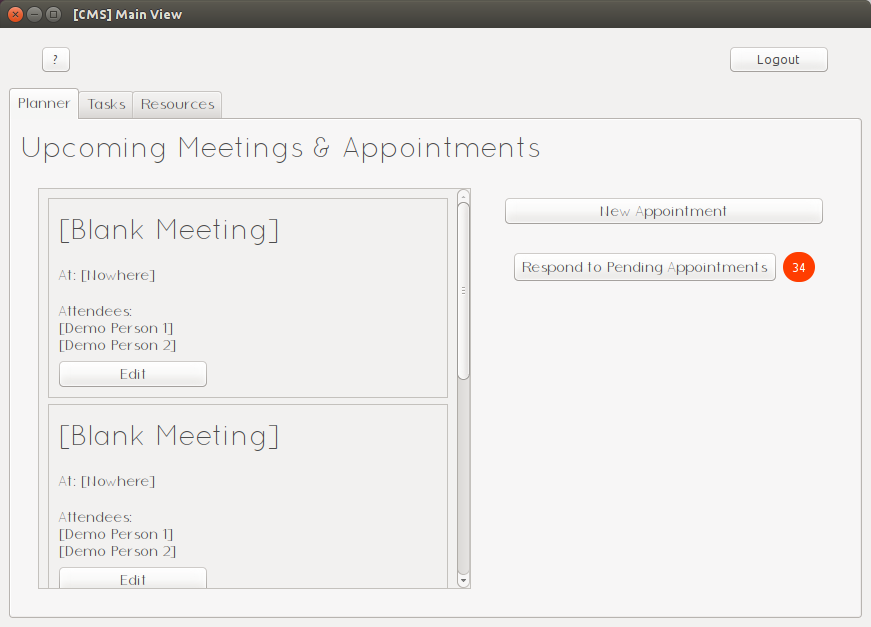
\includegraphics[width=\textwidth]{./Design/proto/2.png}
	\end{figure}
	\begin{figure}[H]
		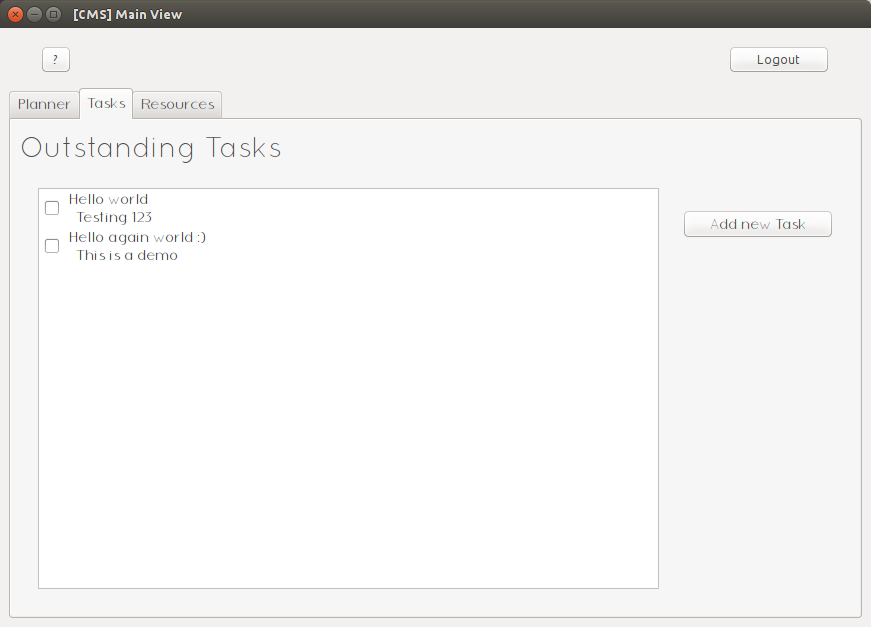
\includegraphics[width=\textwidth]{./Design/proto/3.png}
	\end{figure}
	\begin{figure}[H]
		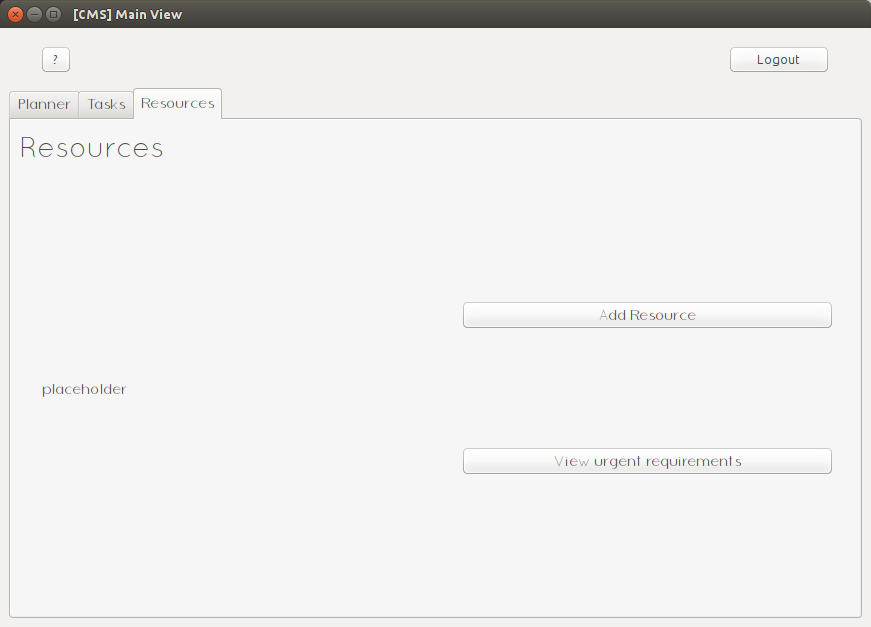
\includegraphics[width=\textwidth]{./Design/proto/4.png}
	\end{figure}
	\begin{figure}[H]
		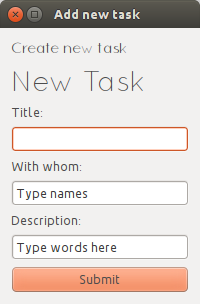
\includegraphics[width=\textwidth]{./Design/proto/5.png}
	\end{figure}
	\begin{figure}[H]
		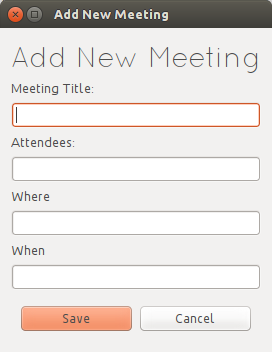
\includegraphics[width=\textwidth]{./Design/proto/6.png}
	\end{figure}
	\begin{figure}[H]
		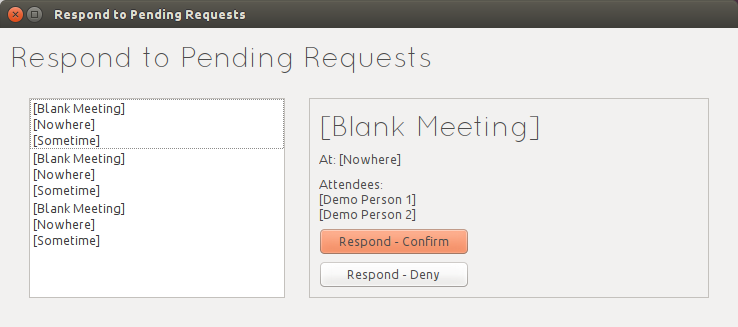
\includegraphics[width=\textwidth]{./Design/proto/7.png}
	\end{figure}
% TODO: Add screenshots from the implementation

\section{Definition of Data Requirements}

\subsection{Identification of all data input items}

\subsection{Identification of all data output items}

\subsection{Explanation of how data output items are generated}

\subsection{Data Dictionary}

% TODO: Define based on Database design

\subsection{Identification of appropriate storage media}

	Because there is potential for there to be a large amount of data, which is likely to be changed and updated frequently, a single non RAID
	spinning HDD would be ample to store the data, because the system is only going to be accessed by a maximum of 10 users simultaneously, speed
	increasing RAID	is not necessary, however a redundancy drive would be useful to provide a continuous backup of the data. Solid state drives
	would not be appropriate because of the continuous reqriting of storage loactions which  would relatively quickly wear out a solid state disk
	which would not be cost effective to replace.

\section{Database Design}

\subsection{Normalisation}

\subsubsection{ER Diagrams}
	\begin{figure}[H]
		\inlcudegraphics[width=\textwidth]{./Design/diagrams/orld.jpg}
		%TODO: this needs to be redone
	\end{figure}

\subsubsection{Entity Descriptions}
User(\underline{UserID}, UserFirstname, UserLastname, UserPasswordHash, Permissions)

Meeting(\underline{MeetingID}, MeetingOwner, MeetingTitle, MeetingDateTime, MeetingPlace, MeetingAttendees)

UserMeeting(\underline{UserID}, \underline{MeetingID}, UserMeetingConfirmation)

Task(\underline{TaskID}, TaskTitle, TaskDescription, TaskOwner, TaskAttendees, TaskExpiry, Priority)

Resource(\underline{ResourceID}, ResourceName, ResourceCost, ResourceQuantity, ResourceRequiredQuantity)

\subsubsection{1NF to 3NF}

	%TODO: make up some non normalised stuff then show the Normalisation process.

\subsection{SQL Queries}
	%TODO: mention output


\section{Security and Integrity of the System and Data}

\subsection{Security and Integrity of Data}
	The sensitive data, as defined under the data protectoin act (personal data such as dates of birth, addresses, contact details; and
	trusted information, such as referral notes or prayer requests) will be encrypted using a two-way encryption algorithm, such as the
	AES algorithm.
	The user's passwords that they use to access this sensitive data will be encrypted using a one-way hashing algorithm, such as the SHA1
	algorithm, so that if the database is accessed using a 3rd party application, the attacker will not be able to read the passwords and
	access the rest of the information using them.


\subsection{System Security}
	The system is protected by a combination of username-password authentication and a user privelleges system, where the administrator can
	change which subsystems each user has access to. Because the system uses a local database file, there is no builtin authentication for
	the data, if the system were to make use of a cloud system, such as Microsoft Azure, this problem would be avoided because of password
	protected  access to the database.

\section{Validation}
	%TODO: how tf do i do this?

\section{Testing}

\begin{landscape}
\subsection{Outline Plan}

\begin{center}
    \begin{tabular}{|p{2cm}|p{5cm}|p{5cm}|p{4cm}|}
        \hline
        \textbf{Test Series} & \textbf{Purpose of Test Series} & \textbf{Testing Strategy} & \textbf{Strategy Rationale}\\ \hline
        Example & Example & Example & Example \\ \hline
    \end{tabular}
\end{center}

\subsection{Detailed Plan}

\begin{center}
    \begin{longtable}{|p{1.5cm}|p{2.5cm}|p{2.5cm}|p{2cm}|p{2cm}|p{2cm}|p{2cm}|p{2cm}|}
        \hline
        \textbf{Test Series} & \textbf{Purpose of Test} & \textbf{Test Description} & \textbf{Test Data} & \textbf{Test Data Type (Normal/ Erroneous/ Boundary)} & \textbf{Expected Result} & \textbf{Actual Result} & \textbf{Evidence}\\ \hline
        Example & Example & Example & Example & Example & Example & Example & Example \\ \hline
    \end{longtable}
\end{center}
\end{landscape}
